\documentclass[border=16pt]{standalone}
\usepackage[T1]{fontenc}
\usepackage{helvet}
\renewcommand{\familydefault}{\sfdefault}
\usepackage{amsmath,amssymb}
\usepackage{tikz}
\usetikzlibrary{arrows.meta,positioning,calc,fit,backgrounds}

% Color palette
\definecolor{ink}{HTML}{0F172A}
\definecolor{subink}{HTML}{334155}

\definecolor{envfill}{HTML}{EFF6FF}
\definecolor{envdraw}{HTML}{2563EB}

\definecolor{visfill}{HTML}{FEF3C7}
\definecolor{visdraw}{HTML}{D97706}

\definecolor{lptcfill}{HTML}{E0F2FE}
\definecolor{lptcdraw}{HTML}{0284C7}

\definecolor{cxfill}{HTML}{FDF2F8}
\definecolor{cxdraw}{HTML}{DB2777}

\definecolor{headfill}{HTML}{ECFDF5}
\definecolor{headdraw}{HTML}{059669}

\definecolor{actfill}{HTML}{FFF7ED}
\definecolor{actdraw}{HTML}{EA580C}

\definecolor{critfill}{HTML}{F1F5F9}
\definecolor{critdraw}{HTML}{475569}

\definecolor{gradred}{HTML}{DC2626}

\begin{document}
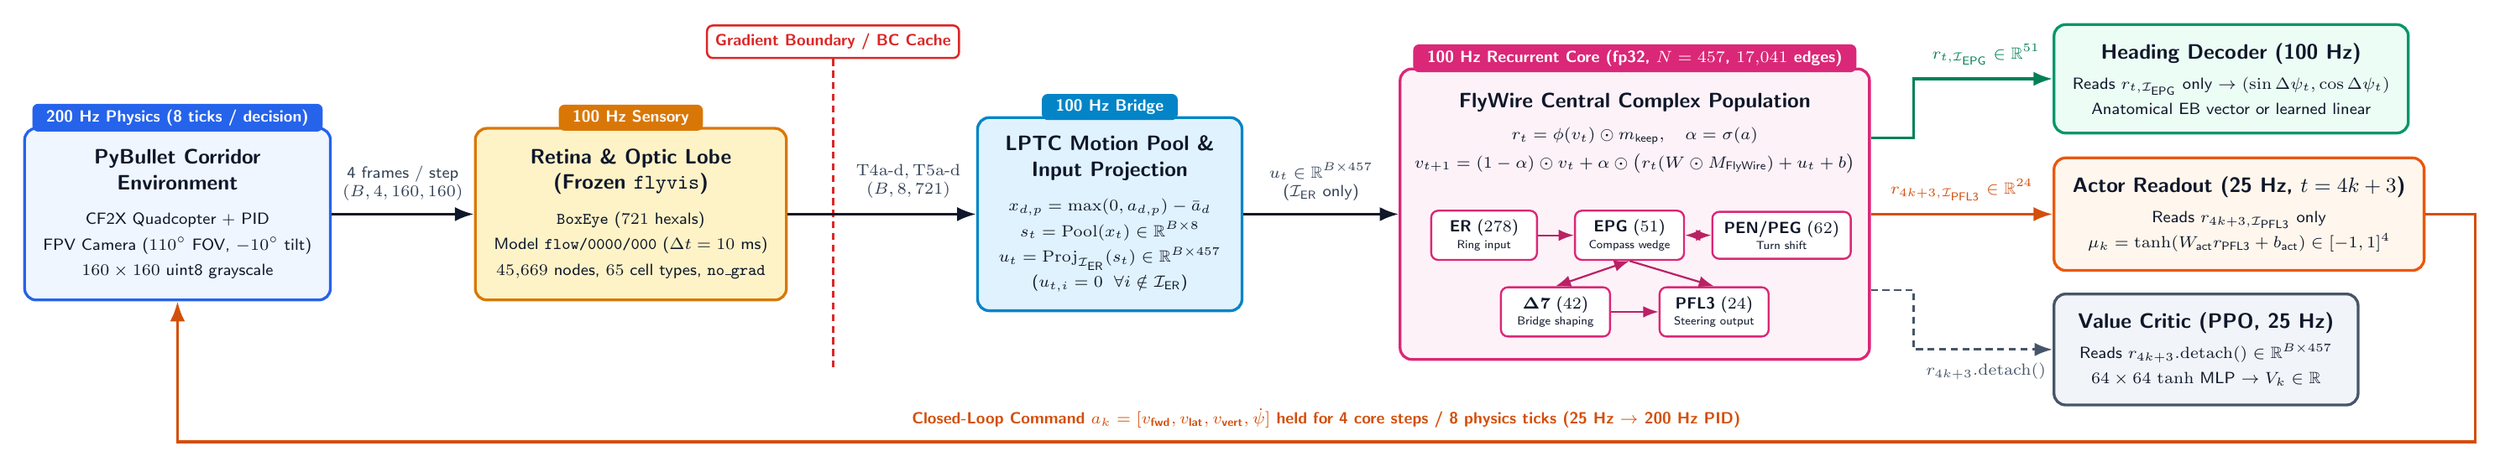
\begin{tikzpicture}[
    font=\sffamily\small,
    >=Latex,
    box/.style={
        rectangle,
        rounded corners=5pt,
        draw=#1,
        line width=1.2pt,
        fill=#1!10,
        text=ink,
        align=center,
        inner sep=8pt
    },
    pill/.style={
        rectangle,
        rounded corners=3pt,
        draw=#1,
        line width=0.85pt,
        fill=white,
        text=ink,
        align=center,
        inner xsep=5pt,
        inner ysep=4pt,
        font=\sffamily\scriptsize
    },
    clocktag/.style={
        rectangle,
        rounded corners=2.5pt,
        fill=ink,
        text=white,
        font=\sffamily\bfseries\scriptsize,
        inner xsep=6pt,
        inner ysep=2.5pt
    },
    arr/.style={
        ->,
        line width=1.15pt,
        draw=ink
    },
    dasharr/.style={
        ->,
        line width=1.05pt,
        densely dashed,
        draw=critdraw
    },
    lbl/.style={
        font=\sffamily\scriptsize,
        text=subink,
        align=center
    }
]

% ================= NODES =================

% 1. PyBullet Corridor Env
\node[box=envdraw, fill=envfill, minimum width=3.6cm, minimum height=2.6cm] (env) at (0, 0) {
    \textbf{PyBullet Corridor}\\
    \textbf{Environment}\\[4pt]
    {\scriptsize CF2X Quadcopter + PID}\\
    {\scriptsize FPV Camera ($110^\circ$ FOV, $-10^\circ$ tilt)}\\
    {\scriptsize $160 \times 160$ uint8 grayscale}
};
\node[clocktag, fill=envdraw] at ($(env.north)+(0,0.14)$) {200 Hz Physics (8 ticks / decision)};

% 2. BoxEye + Frozen flyvis
\node[box=visdraw, fill=visfill, minimum width=3.9cm, minimum height=2.6cm, right=2.15cm of env] (flyvis) {
    \textbf{Retina \& Optic Lobe}\\
    \textbf{(Frozen \texttt{flyvis})}\\[4pt]
    {\scriptsize \texttt{BoxEye} ($721$ hexals)}\\
    {\scriptsize Model \texttt{flow/0000/000} ($\Delta t = 10\text{ ms}$)}\\
    {\scriptsize $45{,}669$ nodes, $65$ cell types, \texttt{no\_grad}}
};
\node[clocktag, fill=visdraw] at ($(flyvis.north)+(0,0.14)$) {100 Hz Sensory};

% 3. LPTC Bridge & Input Projection
\node[box=lptcdraw, fill=lptcfill, minimum width=4.0cm, minimum height=2.6cm, right=2.85cm of flyvis] (lptc) {
    \textbf{LPTC Motion Pool \&}\\
    \textbf{Input Projection}\\[4pt]
    {\scriptsize $x_{d,p} = \max(0, a_{d,p}) - \bar{a}_d$}\\
    {\scriptsize $s_t = \mathrm{Pool}(x_t) \in \mathbb{R}^{B \times 8}$}\\
    {\scriptsize $u_t = \mathrm{Proj}_{\mathcal{I}_{\text{ER}}}(s_t) \in \mathbb{R}^{B \times 457}$}\\
    {\scriptsize ($u_{t,i} = 0\;\;\forall i \notin \mathcal{I}_{\text{ER}}$)}
};
\node[clocktag, fill=lptcdraw] at ($(lptc.north)+(0,0.14)$) {100 Hz Bridge};

% 4. Central Complex Core
\node[box=cxdraw, fill=cxfill, minimum width=7.1cm, minimum height=4.4cm, right=2.35cm of lptc] (cx) {};
\node[clocktag, fill=cxdraw] at ($(cx.north)+(0,0.14)$) {100 Hz Recurrent Core (fp32, $N = 457$, $17{,}041$ edges)};

\node[anchor=north, text=ink, align=center] at ($(cx.north)+(0,-0.26)$) {
    \textbf{FlyWire Central Complex Population}\\[3pt]
    {\scriptsize $r_t = \phi(v_t) \odot m_{\text{keep}}, \quad \alpha = \sigma(a)$}\\[1pt]
    {\scriptsize $v_{t+1} = (1-\alpha)\odot v_t + \alpha\odot\big(r_t(W \odot M_{\text{FlyWire}}) + u_t + b\big)$}
};

% Internal cell-type pills inside CX
\node[pill=cxdraw, minimum width=1.60cm] (g_er)  at ($(cx.center)+(-2.28, -0.32)$) {\textbf{ER} ($278$)\\[-1pt]{\tiny Ring input}};
\node[pill=cxdraw, minimum width=1.65cm] (g_epg) at ($(cx.center)+(-0.08, -0.32)$) {\textbf{EPG} ($51$)\\[-1pt]{\tiny Compass wedge}};
\node[pill=cxdraw, minimum width=1.75cm] (g_pen) at ($(cx.center)+(2.22,  -0.32)$) {\textbf{PEN/PEG} ($62$)\\[-1pt]{\tiny Turn shift}};

\node[pill=cxdraw, minimum width=1.65cm] (g_d7)  at ($(cx.center)+(-1.20, -1.48)$) {$\mathbf{\Delta 7}$ ($42$)\\[-1pt]{\tiny Bridge shaping}};
\node[pill=cxdraw, minimum width=1.65cm] (g_pfl) at ($(cx.center)+(1.20,  -1.48)$) {\textbf{PFL3} ($24$)\\[-1pt]{\tiny Steering output}};

\draw[->, draw=cxdraw!85!black, line width=0.8pt] (g_er.east) -- (g_epg.west);
\draw[<->, draw=cxdraw!85!black, line width=0.8pt] (g_epg.east) -- (g_pen.west);
\draw[<->, draw=cxdraw!85!black, line width=0.8pt] (g_epg.south) -- (g_d7.north);
\draw[->, draw=cxdraw!85!black, line width=0.8pt] (g_epg.south) -- (g_pfl.north);
\draw[->, draw=cxdraw!85!black, line width=0.8pt] (g_d7.east) -- (g_pfl.west);

% 5. Readout Heads (Right column)
\node[box=headdraw, fill=headfill, minimum width=4.6cm, minimum height=1.45cm, right=2.75cm of cx, yshift=2.05cm] (head) {
    \textbf{Heading Decoder (100 Hz)}\\[2pt]
    {\scriptsize Reads $r_{t, \mathcal{I}_{\text{EPG}}}$ only $\to (\sin\Delta\psi_t, \cos\Delta\psi_t)$}\\
    {\scriptsize Anatomical EB vector or learned linear}
};

\node[box=actdraw, fill=actfill, minimum width=4.6cm, minimum height=1.45cm, right=2.75cm of cx] (actor) {
    \textbf{Actor Readout (25 Hz, $t = 4k+3$)}\\[2pt]
    {\scriptsize Reads $r_{4k+3, \mathcal{I}_{\text{PFL3}}}$ only}\\
    {\scriptsize $\mu_k = \tanh(W_{\text{act}} r_{\text{PFL3}} + b_{\text{act}}) \in [-1, 1]^4$}
};

\node[box=critdraw, fill=critfill, minimum width=4.6cm, minimum height=1.45cm, right=2.75cm of cx, yshift=-2.05cm] (critic) {
    \textbf{Value Critic (PPO, 25 Hz)}\\[2pt]
    {\scriptsize Reads $r_{4k+3}.\mathrm{detach}() \in \mathbb{R}^{B \times 457}$}\\
    {\scriptsize $64 \times 64$ $\tanh$ MLP $\to V_k \in \mathbb{R}$}
};

% ================= CONNECTIONS =================

% Env -> flyvis
\draw[arr] (env.east) -- node[above=2pt, lbl] {4 frames / step\\$(B, 4, 160, 160)$} (flyvis.west);

% Gradient boundary & BC Cache between flyvis and LPTC
\coordinate (gb_mid) at ($(flyvis.east)!0.24!(lptc.west)$);
\coordinate (gb_top) at ($(gb_mid)+(0, 2.35)$);
\coordinate (gb_bot) at ($(gb_mid)+(0, -2.35)$);
\draw[densely dashed, line width=1.25pt, draw=gradred] (gb_top) -- (gb_bot);
\node[fill=white, draw=gradred, line width=0.9pt, rounded corners=2.5pt, inner sep=3.5pt, font=\sffamily\bfseries\scriptsize, text=gradred, anchor=south] at (gb_top) {Gradient Boundary / BC Cache};

% flyvis -> LPTC
\draw[arr] (flyvis.east) -- node[pos=0.64, above=3pt, lbl] {$\mathrm{T4a\text{-}d}, \mathrm{T5a\text{-}d}$\\$(B, 8, 721)$} (lptc.west);

% LPTC -> CX
\draw[arr] (lptc.east) -- node[above=2pt, lbl] {$u_t \in \mathbb{R}^{B \times 457}$\\($\mathcal{I}_{\text{ER}}$ only)} (cx.west);

% CX -> Readouts
\coordinate (cx_head_out) at ($(cx.east)+(0, 1.15)$);
\coordinate (cx_crit_out) at ($(cx.east)+(0, -1.15)$);

\draw[arr, draw=headdraw!85!black] (cx_head_out) -- ($(cx_head_out)+(0.65, 0)$) |-
    node[pos=0.76, above=2pt, lbl, text=headdraw!85!black] {$r_{t, \mathcal{I}_{\text{EPG}}} \in \mathbb{R}^{51}$} (head.west);

\draw[arr, draw=actdraw!90!black] (cx.east) --
    node[above=2pt, lbl, text=actdraw!90!black] {$r_{4k+3, \mathcal{I}_{\text{PFL3}}} \in \mathbb{R}^{24}$} (actor.west);

\draw[dasharr] (cx_crit_out) -- ($(cx_crit_out)+(0.65, 0)$) |-
    node[pos=0.76, below=2pt, lbl, text=critdraw] {$r_{4k+3}.\mathrm{detach}()$} (critic.west);

% Closed-loop Action feedback from Actor back to PyBullet Env (routed cleanly below Critic)
\coordinate (fb_right) at ($(actor.east)+(0.75, 0)$);
\coordinate (fb_bot) at (0, -3.45);
\draw[arr, draw=actdraw!90!black, line width=1.25pt] (actor.east) -- (fb_right) |- (fb_bot)
    node[pos=0.75, above=2pt, font=\sffamily\bfseries\scriptsize, text=actdraw!90!black]
    {Closed-Loop Command $a_k = [v_{\text{fwd}}, v_{\text{lat}}, v_{\text{vert}}, \dot{\psi}]$ held for 4 core steps / 8 physics ticks (25 Hz $\to$ 200 Hz PID)}
    -- (env.south);

\end{tikzpicture}
\end{document}
